\documentclass[12pt, letterpaper]{../assignment}
\usepackage{graphicx}
\usepackage{courier}
\usepackage{minted}
\usepackage{amsmath}
\usepackage{commath}
\usepackage{amssymb}
\usepackage{amsfonts} 
\usepackage{cancel}
\usepackage{enumitem}
\usepackage{array}

\usepackage{tikz}
\usetikzlibrary{shapes,arrows,positioning}

\usemintedstyle{monokai}
\oddsidemargin = 0pt
\exercisesheet{Module 6}{Practice Assignment}
\student{Austin Barrilleaux}
\courselabel{EN 525.609}
\semester{Fall 2023}
\usepackage[backend=bibtex,style=numeric,sorting=none]{biblatex}
\bibliography{reference}
\usepackage{color}
\definecolor{light-gray}{rgb}{0.2,0.2,0.2}
\setminted{bgcolor=light-gray}
\setlength{\parindent}{0pt}

\makeatletter
\patchcmd{\minted@colorbg}{\noindent}{\medskip\noindent}{}{}
\apptocmd{\endminted@colorbg}{\par\medskip}{}{}
\makeatother

\begin{document}
\subsection*{Problem 1}
\subsubsection*{Solve the following practice problems in the 9th edition textbook.\\
\begin{itemize}
    \item Chapter 5:
    \begin{itemize}
        \item 5-1 (a,b)
        \item 5-18
        \item 5-19
    \end{itemize}
\end{itemize}}

\subsubsection*{5-1. A pair of complex-conjugate poles in the s-plane is required to meet the various specifications that follow.
For each specification, sketch the region in the s-plane in which the poles should be located.}

\subsubsection*{(a) $\zeta \ge 0.707 $, $\omega_n \ge 2$ rad/sec, (positive damping)}

The following sketch shows the region in the s-plane in which the poles should be located (hand shaded area in black):

\begin{figure}[H]
    \centering
    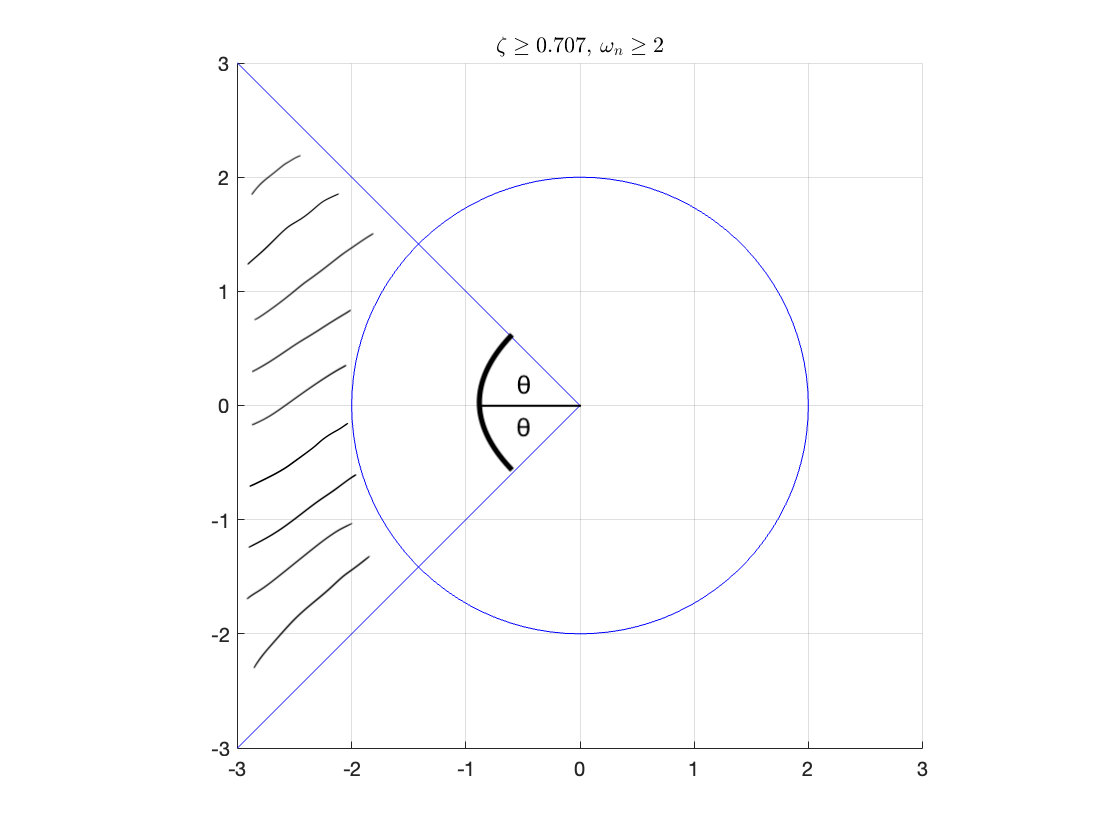
\includegraphics[width=0.7\linewidth]{./figures/problem_5_1_a.png}
    % \caption{Step Response}
    \label{fig:step}
\end{figure}

The plot was generated using MATLAB then annotated.

The value for $\theta$ was calculated as:

$$ \theta = \cos^{-1}(\zeta) = \cos^{-1}(0.707) = 0.7855 $$

This value for $\theta$ which is in radians is roughly equal to 45 degrees.

\subsubsection*{(a) $0 \le \zeta \le 0.707 $, $\omega_n \le 2$ rad/sec, (positive damping)}

The following sketch shows the region in the s-plane in which the poles should be located (hand shaded area in black):

\begin{figure}[H]
    \centering
    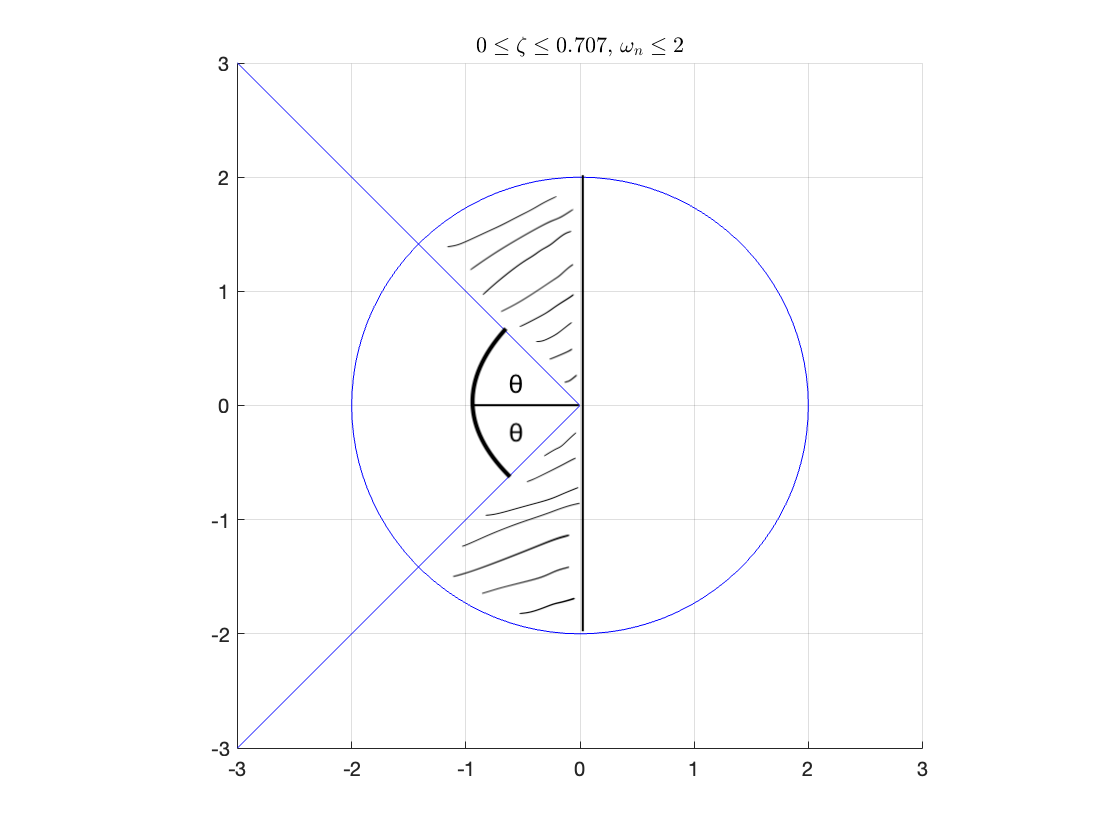
\includegraphics[width=0.7\linewidth]{./figures/problem_5_1_b.png}
    % \caption{Step Response}
    \label{fig:step}
\end{figure}

The value for $\theta$, was calculated the same as in part (a),
as the boundary of the region was the same.

\subsubsection*{5-18. The unit-step response of a linear control system is shown in Fig. SP- I8. Find the transfer
function of a second-order prototype system to model the system.}

\begin{figure}[H]
    \centering
    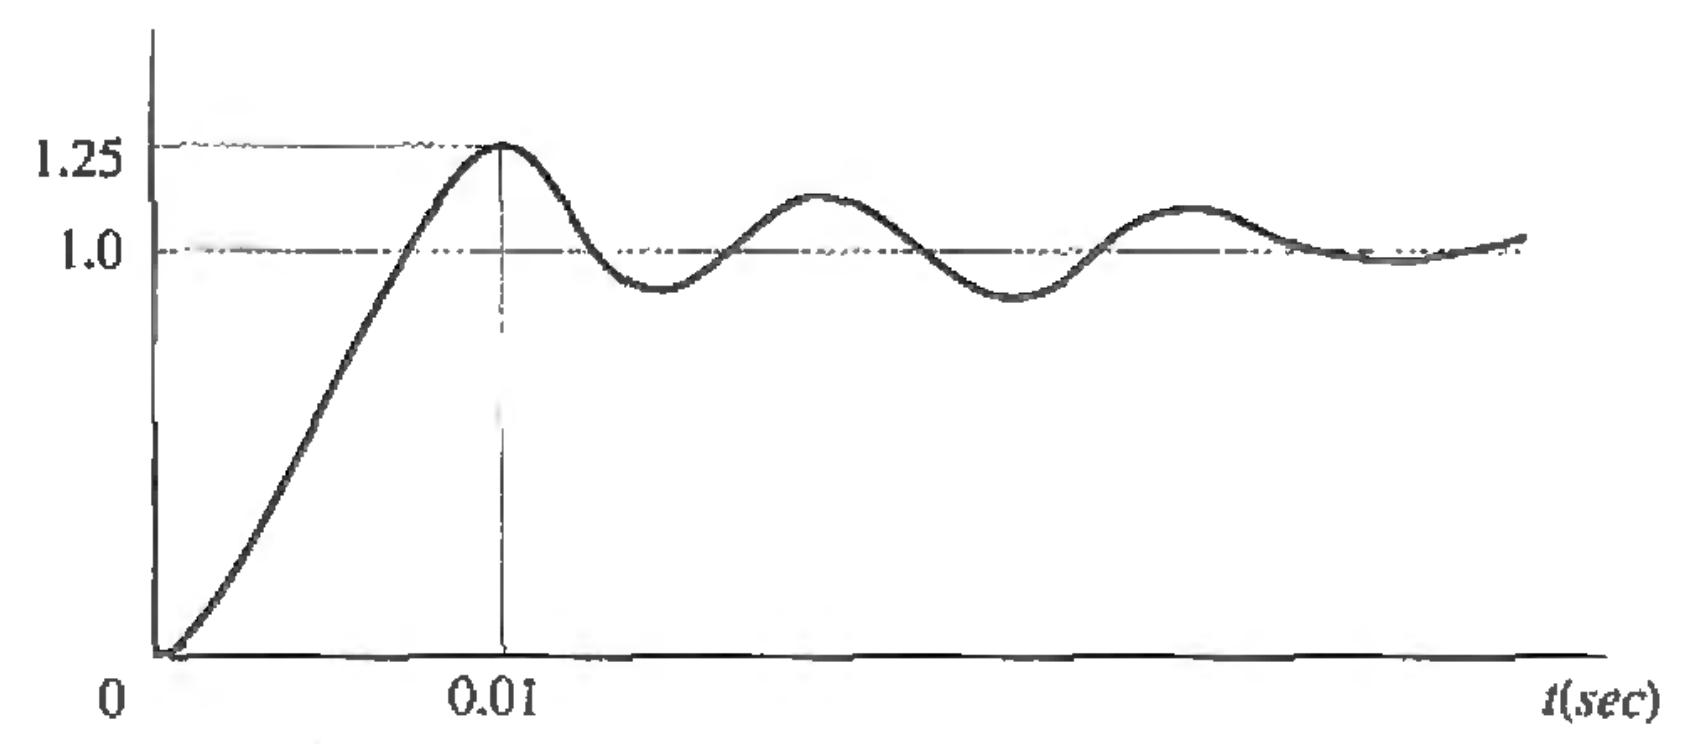
\includegraphics[width=0.7\linewidth]{./figures/problem_5_18.png}
    % \caption{Step Response}
    \label{fig:step}
\end{figure}

We know that the equation for maximum overshoot is:

$$ y(t_p) - 1 = e^\frac{-\pi \zeta}{\sqrt{1 - \zeta^2}} $$

Populating that $ y(t_p) = 1.25 $, the equation can be written as:

$$ 0.25 = e^\frac{-\pi \zeta}{\sqrt{1 - \zeta^2}} $$

Further, taking the natural log of both sides:

$$ \text{ln}(0.25) = \frac{-\pi \zeta}{\sqrt{1 - \zeta^2}} $$

Reorganizing this:

$$ \text{ln}(0.25)^2 (1 - \zeta^2) = \pi^2 \zeta^2 $$

Solving for $zeta$, we get:

$$ \text{ln}(0.25)^2 = (\text{ln}(0.25)^2 + \pi^2) \zeta^2 $$

Further:

$$ \zeta^2 = \frac{\text{ln}(0.25)^2}{(\text{ln}(0.25)^2 + \pi^2)} $$

Or:

$$ \zeta = \sqrt{\frac{\text{ln}(0.25)^2}{(\text{ln}(0.25)^2 + \pi^2)}} \approx 0.4037 $$

Which evaluated in MATLAB is approximately $ \zeta \approx 0.4037 $.
\\\\
Now that we have $\zeta$, using the following equation for peak time, we can solve for $\omega_n$:

$$ t_p = \frac{\pi}{\omega_n \sqrt{1-\zeta^2}} $$

Re-arranging:

$$ \omega_n = \frac{\pi}{ t_p \sqrt{1-\zeta^2}} $$

Solving this in MATLAB using the solved value of $\zeta$, the value for $\omega_n$ is:

$$ \omega_n = \frac{\pi}{ 0.01 \sqrt{1-\zeta^2}} \approx 343.3863\ \ \text{rad/s} $$

The gives a transfer function of:

$$ \frac{Y(s)}{R(s)} = \frac{\omega_n^2}{s^2 + 2 \zeta \omega_n s + \omega_n^2 } = \frac{117914.16}{s^2 + 277.25s + 117914.16 } $$

The final result is:
\begin{answer}
$$ \frac{Y(s)}{R(s)} = \frac{117914.16}{s^2 + 277.25s + 117914.16 } $$
\end{answer}

The following MATLAB script provides this answer:

\color{white}
\hspace*{6em}\inputminted[frame=leftline,fontsize=\footnotesize]{matlab}
{./matlab/Problem_5_18.m}
\color{black}

\subsubsection*{5-19. For the control system shown in Fig. 5P-13, find the values of $K$ and $K_t$,
so that the maximum overshoot of the output is approximately 4.3\% and the rise time $t_r$,
is approximately 0.2 sec. Simulate the system with any time-response simulation program to check the accuracy of your solutions.}

\begin{figure}[H]
    \centering
    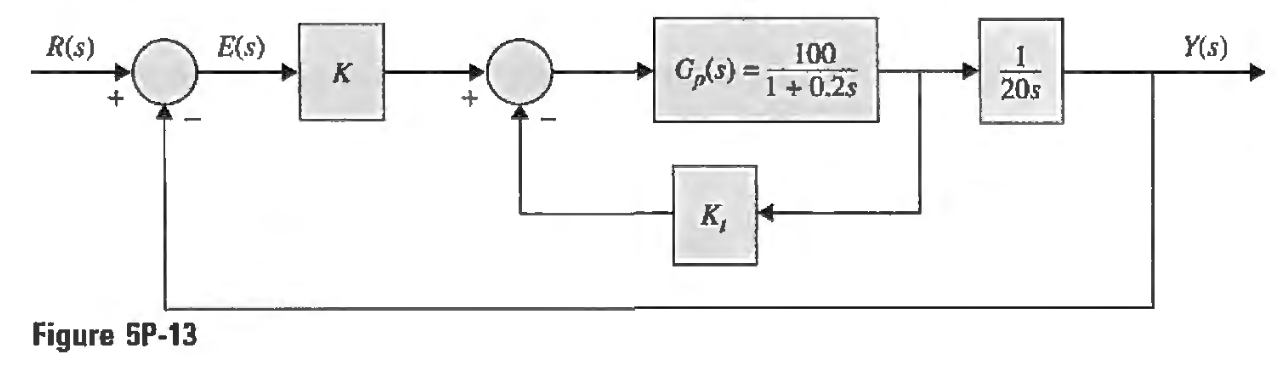
\includegraphics[width=0.7\linewidth]{./figures/problem_5_19.png}
    % \caption{Step Response}
    \label{fig:step}
\end{figure}

This block diagram reduces to:

$$ \frac{Y(s)}{R(s)} = \frac{100 K}{4 s^2 + 20s + 2000 K_t s + 100 K } = \frac{25 K}{ s^2 + (5 + 500 K_t) s + 25 K } $$

Putting this into the form:

$$ \frac{Y(s)}{R(s)} = \frac{\omega_n^2}{s^2 + 2 \zeta \omega_n s + \omega_n^2 } $$

This means that:

$$ \omega_n  = 5 \sqrt{K} $$

$$ 2 \zeta \omega_n =  (5 + 500 K_t) $$

Populating the latter function with $\omega_n$:

$$ \zeta =  \frac{(0.5 + 50 K_t)}{sqrt{K}} $$

Since:

$$ y(t_p) - 1 = e^\frac{-\pi \zeta}{\sqrt{1 - \zeta^2}} $$

Populating that $ y(t_p) = 1.25 $, the equation can be written as:

$$ 0.043 = e^\frac{-\pi \zeta}{\sqrt{1 - \zeta^2}} $$

Further, taking the natural log of both sides:

$$ \text{ln}(0.043) = \frac{-\pi \zeta}{\sqrt{1 - \zeta^2}} $$

Reorganizing this:

$$ \text{ln}(0.043)^2 (1 - \zeta^2) = \pi^2 \zeta^2 $$

Solving for $zeta$, we get:

$$ \text{ln}(0.043)^2 = (\text{ln}(0.043)^2 + \pi^2) \zeta^2 $$

Further:

$$ \zeta^2 = \frac{\text{ln}(0.043)^2}{(\text{ln}(0.043)^2 + \pi^2)} $$

Or:

$$ \zeta = \sqrt{\frac{\text{ln}(0.043)^2}{(\text{ln}(0.043)^2 + \pi^2)}} \approx 0.7077 $$

Given this value for $\zeta$ we can now solve for $\omega_n$ using:

$$ t_r = \frac{ 1 - 0.4167 \zeta + 2.917 \zeta^2 }{\omega_n} $$

Re-arranging:

$$ \omega_n = \frac{ 1 - 0.4167 \zeta + 2.917 \zeta^2 }{t_r} $$

Solving this in MATLAB using the solved value of $\zeta$, the value for $\omega_n$ is:

$$ \omega_n = \frac{ 1 - 0.4167 \cdot 0.7077 + 2.917 \cdot 0.7077^2 }{t_r} \approx 10.83\ \ \text{rad/s} $$

Since $ \omega_n  = 5 \sqrt{K} $, this means that:
\begin{answer}
$$ K = \frac{\omega_n ^2}{25} = \frac{10.83 ^2}{25} \approx 4.69 $$
\end{answer}

Using this value of $K$, we can now solve for $K_t$:

$$ \zeta =  \frac{(0.5 + 50 K_t)}{sqrt{K}} $$

Re-arranging:
\begin{answer}
$$ K_t = \frac{\zeta \sqrt{K} - 0.5}{50} \approx 0.0207 $$
\end{answer}

Using this to populate the transfer function, we get:

\begin{answer}
$$ \frac{Y(s)}{R(s)} =  \frac{25 \cdot 4.69 }{ s^2 + (5 + 500 \cdot 0.0207) s + 25 \cdot 4.69 } $$
\end{answer}

Plotting the step response using the \texttt{step()} function in MATLAB, we get the following response:


\begin{figure}[H]
    \centering
    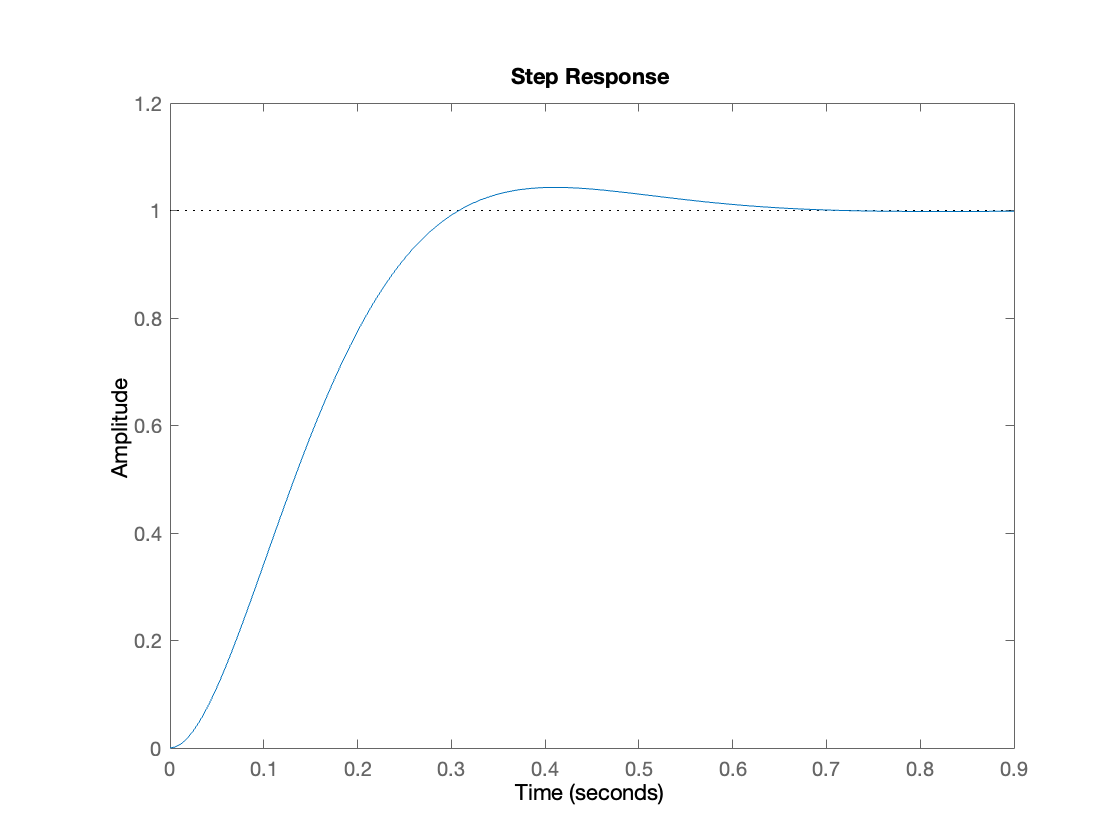
\includegraphics[width=0.7\linewidth]{./figures/problem_5_19_result.png}
    % \caption{Step Response}
    \label{fig:step}
\end{figure}

The max $y$ value of the response is $y = 1.04299$, or an overshoot of 4.299\%. The rise time is 0.1979 sec.
\\\\
The following MATLAB script provides these answers:

\color{white}
\hspace*{6em}\inputminted[frame=leftline,fontsize=\footnotesize]{matlab}
{./matlab/Problem_5_19.m}
\color{black}

\subsection*{Problem 1}
\subsubsection*{Consider the following block diagram of a missile attitude control system:}

\begin{figure}[H]
    \centering
    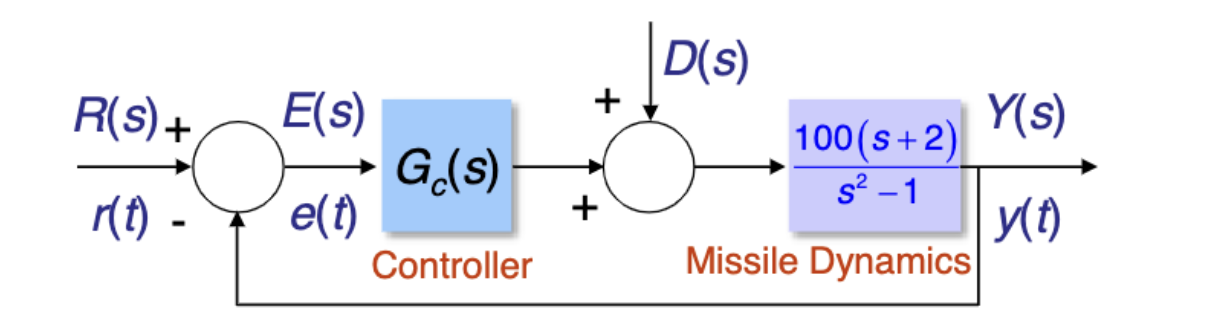
\includegraphics[width=0.7\linewidth]{./figures/missile_system.png}
    % \caption{Step Response}
    \label{fig:step}
\end{figure}

\subsubsection*{For, $G_c(s)=(s+\alpha)/s$,
use MATLAB to plot the step responses of the
system for $\alpha=5, 50 \ \text{and}\  500$,
and comment on the step response of the three cases (assume zero I.C.'s)}

The transfer function for this system is:

$$ \frac{Y(s)}{R(s)} = \frac{100 s^2 + (200 + 100\alpha) s +200\alpha}{s^3 + 100 s^2 + (199 + 100 \alpha) s + 200 \alpha} $$

Plotting these in MATLAB, we get the following responses:

\begin{figure}[H]
    \centering
    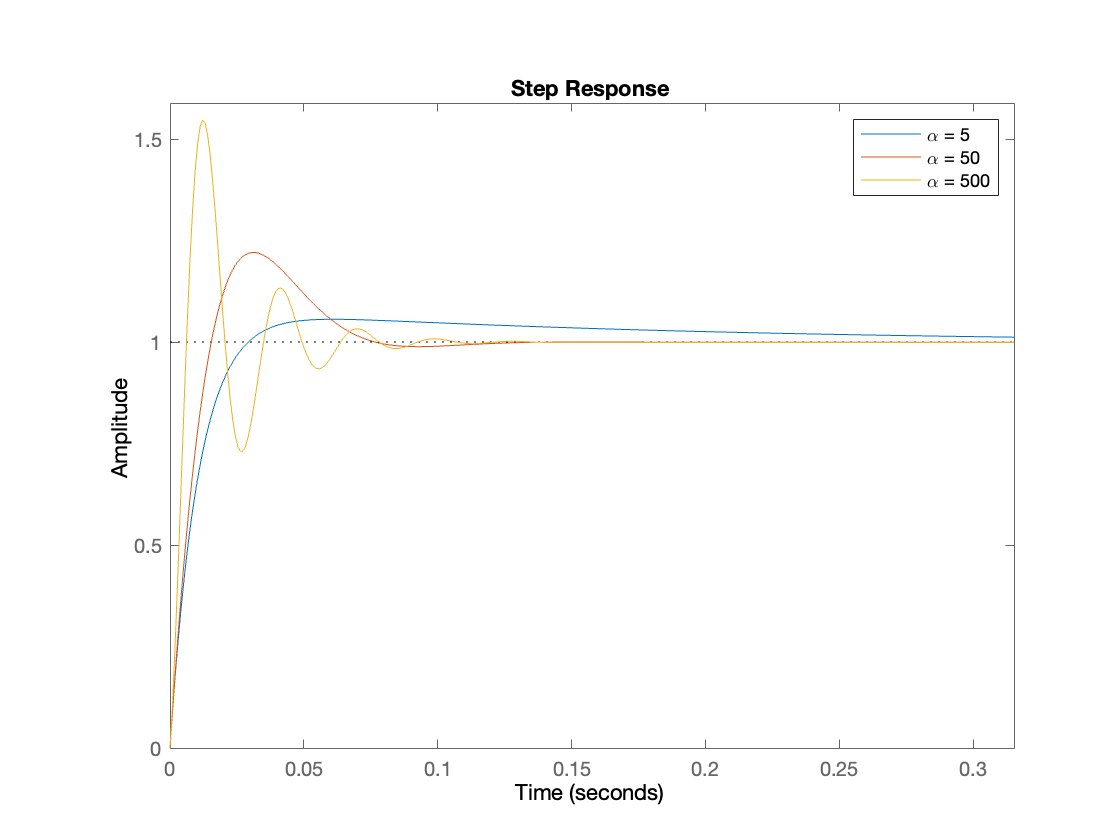
\includegraphics[width=0.8\linewidth]{./figures/Problem_2.png}
    % \caption{Step Response}
    \label{fig:step}
\end{figure}

The poles of each response are included in the following figure:

\begin{figure}[H]
    \centering
    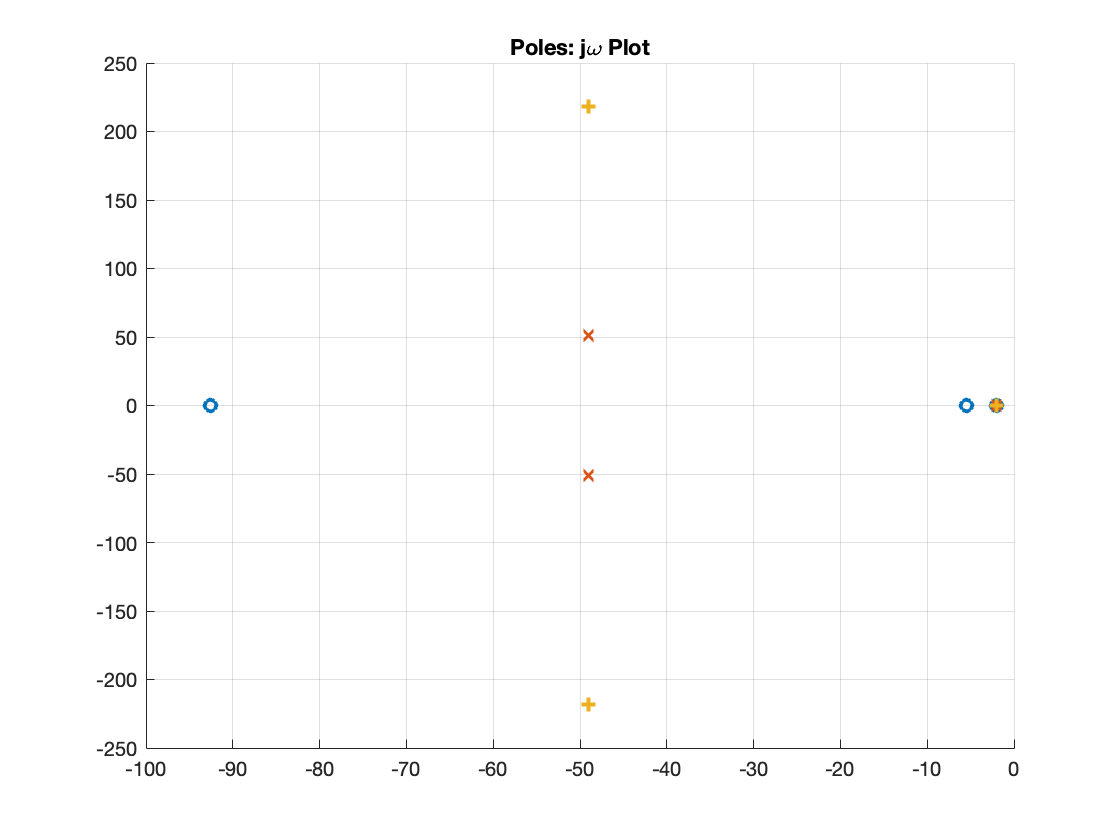
\includegraphics[width=0.7\linewidth]{./figures/Problem_2_roots.png}
    % \caption{Step Response}
    \label{fig:step}
\end{figure}

\begin{answer}
\bf{
When $\alpha  = 5$, the system has only real poles (no complex poles). The system is slightly under-damped, with low overshoot.
When $\alpha  = 50$, the system has one real pole near zero, and a complex conjugate pair to the left of the real pole.
The dominant pole for $\alpha = 50$ is slightly to the left of $\alpha = 5$.
As this pole moved to the left, rise time and overshoot increase.
This behavior relative to the dominant pole increases more for the case $\alpha = 500$, as it moves further left.
For $\alpha = 500$ the complex conjugate pair has larger imaginary values (a larger $\omega_n$),
driving a much more transient response than $\alpha = 50$.
}
\end{answer}

% $$ \frac{Y(s)}{R(s)} = \frac{\omega_n^2}{s^2 + 2 \zeta \omega_n s + \omega_n^2 } = \frac{117914.16}{s^2 + 277.25s + 117914.16 } $$

% The final result is:
% \begin{answer}
% $$ \frac{Y(s)}{R(s)} = \frac{117914.16}{s^2 + 277.25s + 117914.16 } $$

% \begin{figure}[H]
%     \centering
%     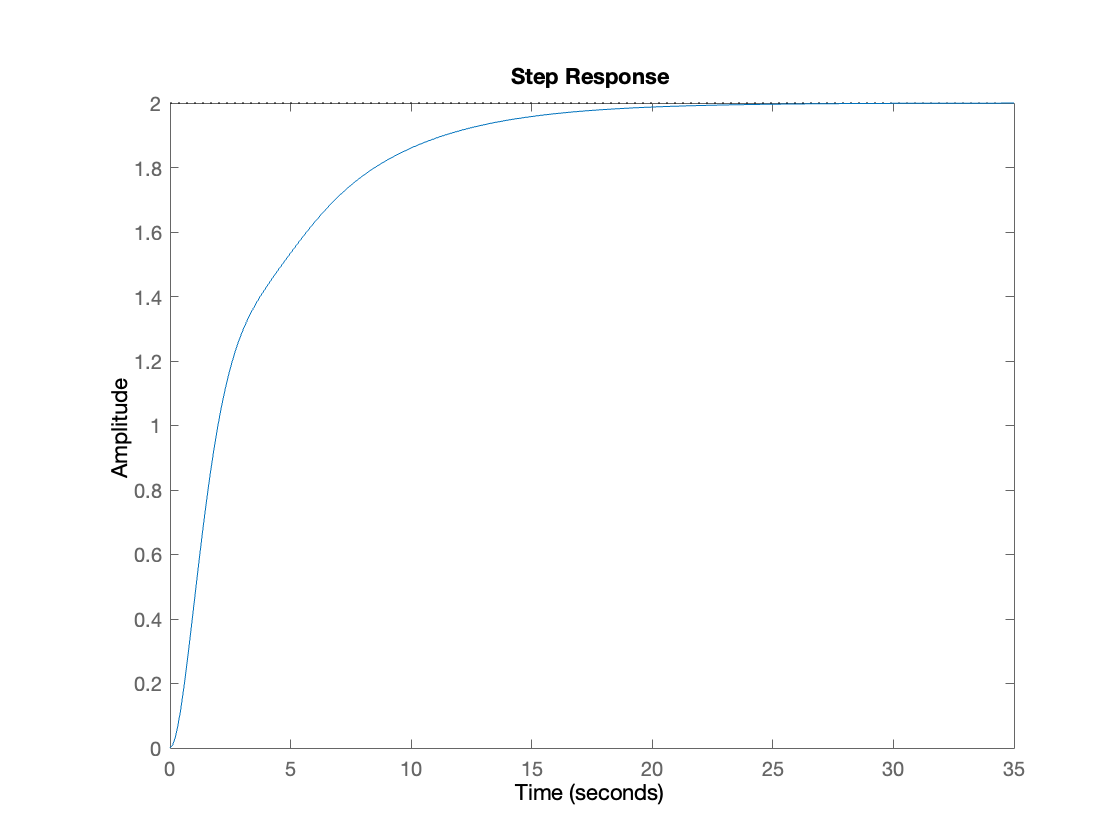
\includegraphics[width=0.7\linewidth]{./figures/step_response.png}
%     \caption{Step Response}
%     \label{fig:step}
%  \end{figure}



\end{document}

